\StartOf{Lecture 22}

\Today{(1) Channel Capacity, (2) Error Correction Coding}

\announcements{
\begin{itemize}
  \item Homework 8 due today at 11:59pm.
  \item Exam 2 is Mon April 20.  Schedule 80 minutes of your day to take this exam.  Most should take it during the class period, but if your schedule / time zone makes this difficult you may pick a different 80 minute period.
\end{itemize}
}


\section{Channel Coding}


\subsection{Review of Source Coding}

In the channel coding lecture, we defined entropy,
\[
  H[X] = -\sum_i p_i \log_2 p_i
\]
and entropy rate,
\[
  H = \lim_{N\rightarrow \infty} \frac{1}{N} H[X_1, X_2, \ldots, X_N].
\]
We showed that entropy can be used to quantify information. Given
our information source $X$ or $\{X_i\}$, the value of $H[X]$ or $H$
gives us a measure of how many bits we need at a minimum to encode the source data without loss.

The major result was the Shannon's source coding theorem, which says
that a source with entropy rate $H$ can be encoded with arbitrarily
small error probability, at any rate $R$ (bits / source output) as
long as $R>H$.  Any lower rate than $H$ would guarantee loss of
information.

\subsection{When we add noise}

Now, we turn to the noisy channel.  This discussion of entropy also allows us to consider the maximum data rate which can be carried without error on a bandlimited channel, which is affected by
additive uncorrelated Gaussian noise.

Ralph V.\ L.\ Hartley (born Nov. 30, 1888) was a researcher for the Western Electric Company, involved in radio telephony, and published a paper in \emph{The Bell System Technical Journal} on ``Transmission of Information'' \cite{hartley1928transmission}.

Hartley was particularly influenced by Nyquist's sampling theorem.  When transmitting a sequence of rectangular pulses, each of duration $T_s$, Nyquist determined that the pulse rate was limited to two times the available channel bandwidth $B$,
\[
  \frac{1}{T_s} \le 2B.
\]
He was considering digital transmission in pulse-amplitude modulated systems.  The pulse rate was limited to $2B$, as described by Nyquist.  But, depending on how pulse amplitudes were chosen, each pulse could represent more or less information.

Hartley assumed that the maximum amplitude available
to the transmitter was $A$ and the minimum amplitude was $0$ (since early receivers were modified AM envelope detectors, and
did not deal well with negative amplitudes).  Then, Hartley made the assumption that
the communication system could discern between pulse amplitudes, if
they were at separated by at least a voltage spacing of $A_\delta$.
Given that a PAM system operates from $0$ to $A$ in increments of
$A_\delta$, as shown in Figure \ref{F:Channel-coding-Hartley}, the number of different pulse amplitudes (symbols) is
\[
  M = 1 + \frac{A}{A_\delta}.
\]

\begin{figure}[htbp]
  \centering{
    


\tikzset{every picture/.style={line width=0.75pt}} %set default line width to 0.75pt        

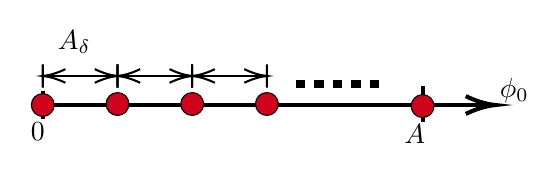
\begin{tikzpicture}[x=0.75pt,y=0.75pt,yscale=-1,xscale=1]
%uncomment if require: \path (0,303); %set diagram left start at 0, and has height of 303

%Straight Lines [id:da1694363996472692] 
\draw [line width=1.5]    (142,207) -- (357,207) ;
\draw [shift={(360,207)}, rotate = 180] [color={rgb, 255:red, 0; green, 0; blue, 0 }  ][line width=1.5]    (14.21,-4.28) .. controls (9.04,-1.82) and (4.3,-0.39) .. (0,0) .. controls (4.3,0.39) and (9.04,1.82) .. (14.21,4.28)   ;
\draw [shift={(142,207)}, rotate = 180] [color={rgb, 255:red, 0; green, 0; blue, 0 }  ][line width=1.5]    (0,6.71) -- (0,-6.71)   ;
%Straight Lines [id:da015408605409965137] 
\draw [line width=1.5]    (325,198) -- (325,215) ;
%Straight Lines [id:da28225347593306416] 
\draw    (142,193) -- (178,193) ;
\draw [shift={(178,193)}, rotate = 180] [color={rgb, 255:red, 0; green, 0; blue, 0 }  ][line width=0.75]    (0,5.59) -- (0,-5.59)(10.93,-3.29) .. controls (6.95,-1.4) and (3.31,-0.3) .. (0,0) .. controls (3.31,0.3) and (6.95,1.4) .. (10.93,3.29)   ;
\draw [shift={(142,193)}, rotate = 0] [color={rgb, 255:red, 0; green, 0; blue, 0 }  ][line width=0.75]    (0,5.59) -- (0,-5.59)(10.93,-3.29) .. controls (6.95,-1.4) and (3.31,-0.3) .. (0,0) .. controls (3.31,0.3) and (6.95,1.4) .. (10.93,3.29)   ;
%Shape: Circle [id:dp08670165967223742] 
\draw  [fill={rgb, 255:red, 208; green, 2; blue, 27 }  ,fill opacity=1 ] (136.5,207) .. controls (136.5,203.96) and (138.96,201.5) .. (142,201.5) .. controls (145.04,201.5) and (147.5,203.96) .. (147.5,207) .. controls (147.5,210.04) and (145.04,212.5) .. (142,212.5) .. controls (138.96,212.5) and (136.5,210.04) .. (136.5,207) -- cycle ;
%Shape: Circle [id:dp17114745324287495] 
\draw  [fill={rgb, 255:red, 208; green, 2; blue, 27 }  ,fill opacity=1 ] (172.5,206.5) .. controls (172.5,203.46) and (174.96,201) .. (178,201) .. controls (181.04,201) and (183.5,203.46) .. (183.5,206.5) .. controls (183.5,209.54) and (181.04,212) .. (178,212) .. controls (174.96,212) and (172.5,209.54) .. (172.5,206.5) -- cycle ;
%Straight Lines [id:da7615059497094845] 
\draw [line width=3]  [dash pattern={on 3.38pt off 3.27pt}]  (264,197) -- (306,197) ;
%Straight Lines [id:da36960417126493583] 
\draw    (178,193) -- (214,193) ;
\draw [shift={(214,193)}, rotate = 180] [color={rgb, 255:red, 0; green, 0; blue, 0 }  ][line width=0.75]    (0,5.59) -- (0,-5.59)(10.93,-3.29) .. controls (6.95,-1.4) and (3.31,-0.3) .. (0,0) .. controls (3.31,0.3) and (6.95,1.4) .. (10.93,3.29)   ;
\draw [shift={(178,193)}, rotate = 0] [color={rgb, 255:red, 0; green, 0; blue, 0 }  ][line width=0.75]    (0,5.59) -- (0,-5.59)(10.93,-3.29) .. controls (6.95,-1.4) and (3.31,-0.3) .. (0,0) .. controls (3.31,0.3) and (6.95,1.4) .. (10.93,3.29)   ;
%Shape: Circle [id:dp29098936246056106] 
\draw  [fill={rgb, 255:red, 208; green, 2; blue, 27 }  ,fill opacity=1 ] (208.5,206.5) .. controls (208.5,203.46) and (210.96,201) .. (214,201) .. controls (217.04,201) and (219.5,203.46) .. (219.5,206.5) .. controls (219.5,209.54) and (217.04,212) .. (214,212) .. controls (210.96,212) and (208.5,209.54) .. (208.5,206.5) -- cycle ;
%Straight Lines [id:da3636038237150647] 
\draw    (214,193) -- (250,193) ;
\draw [shift={(250,193)}, rotate = 180] [color={rgb, 255:red, 0; green, 0; blue, 0 }  ][line width=0.75]    (0,5.59) -- (0,-5.59)(10.93,-3.29) .. controls (6.95,-1.4) and (3.31,-0.3) .. (0,0) .. controls (3.31,0.3) and (6.95,1.4) .. (10.93,3.29)   ;
\draw [shift={(214,193)}, rotate = 0] [color={rgb, 255:red, 0; green, 0; blue, 0 }  ][line width=0.75]    (0,5.59) -- (0,-5.59)(10.93,-3.29) .. controls (6.95,-1.4) and (3.31,-0.3) .. (0,0) .. controls (3.31,0.3) and (6.95,1.4) .. (10.93,3.29)   ;
%Shape: Circle [id:dp32236714952833534] 
\draw  [fill={rgb, 255:red, 208; green, 2; blue, 27 }  ,fill opacity=1 ] (244.5,206.5) .. controls (244.5,203.46) and (246.96,201) .. (250,201) .. controls (253.04,201) and (255.5,203.46) .. (255.5,206.5) .. controls (255.5,209.54) and (253.04,212) .. (250,212) .. controls (246.96,212) and (244.5,209.54) .. (244.5,206.5) -- cycle ;
%Shape: Circle [id:dp7630499866122051] 
\draw  [fill={rgb, 255:red, 208; green, 2; blue, 27 }  ,fill opacity=1 ] (319.5,207.5) .. controls (319.5,204.46) and (321.96,202) .. (325,202) .. controls (328.04,202) and (330.5,204.46) .. (330.5,207.5) .. controls (330.5,210.54) and (328.04,213) .. (325,213) .. controls (321.96,213) and (319.5,210.54) .. (319.5,207.5) -- cycle ;

% Text Node
\draw (148,170) node [anchor=north west][inner sep=0.75pt]    {$A_{\delta }$};
% Text Node
\draw (315,215) node [anchor=north west][inner sep=0.75pt]    {$A$};
% Text Node
\draw (361,193) node [anchor=north west][inner sep=0.75pt]    {$\phi _{0}$};
% Text Node
\draw (135,214) node [anchor=north west][inner sep=0.75pt]    {$0$};


\end{tikzpicture}
  }
  \caption{Hartley assigned symbols (\textcolor{red}{$\bullet$}) in a 1-D non-negative PAM system with maximum amplitude $A$ and distance between neighboring symbols of $A_\delta$.}
  \label{F:Channel-coding-Hartley}
\end{figure}


Next, Hartley used the `bit' measure to quantify the data which
could be encoded using $M$ amplitude levels,
\[
  \log_2 M =  \log_2 \left( 1 + \frac{A}{A_\delta} \right)
\]

Finally, Hartley quantified the data rate using Nyquist's
relationship to determine the maximum rate $R_{max}$, in bits per second,
possible from the digital communication system,
\[
  R_{max} =  2B \log_2 \left( 1 + \frac{A}{A_\delta} \right)
\]


\subsection{C. E. Shannon}

What was left unanswered by Hartley's capacity formula was the relationship between noise and the minimum amplitude separation between symbols.  Engineers would have to be conservative when setting $A_\delta$ to ensure a low probability of error.  Furthermore, the capacity formula was for a particular type of PAM system, and did not say anything fundamental about the relationship between capacity and bandwidth for arbitrary modulation.

\subsubsection{Noisy Channel}

Shannon did take into account an additive uncorrelated Gaussian noise channel, and used statistics to develop a universal bound for capacity, regardless of modulation type \cite{shannon1948mathematical}.  In this channel model, the $i$th symbol sample at the receiver (after the matched filter, assuming perfect synchronization) is $y_i$,
\[
  y_i = x_i + z_i
\]
where $x_i$ is the transmitted signal and $z_i$ is the noise in the
channel.  The noise term $z_i$ is assumed to be i.i.d.~Gaussian with
variance $E_N = N_0/2$.

\subsubsection{Introduction of Latency}

Shannon's key insight was to exchange latency (time delay) for reduced probability of error.  In fact, his capacity bound considers $n$-dimensional signaling.  So the received vector is $\mby = [y_1, \ldots, y_n]$, of length $n$.  These might be truly an $n$-dimensional signal (\eg, FSK or OFDM), or they might use multiple symbols over time (recall that symbols at delays that are multiples of $T_s$ are orthogonal). In either case, Shannon uses all $n$ dimensions in the constellation -- the detector must use all $n$ elements of the $\mby$ vector to make a decision. In the multiple symbols over time, this late decision will decide all values of $\mbx = [x_1, \ldots, x_n]$ simultaneously. Further, Shannon's proof considers the limiting case as $n\rightarrow \infty$.

This asymptotic limit as $n\rightarrow \infty$ allows for a proof using the statistical convergence of a sequence of random variables. In particular, we need a law called \emph{the law of large numbers}.  
This law says that the following event,
\[
  \frac{1}{n} \sum_{i=1}^n (y_i - x_i)^2 \le E_N
\]
happens with probability one, as $n\rightarrow \infty$.  In other words, as $n\rightarrow \infty$, the measured value $\mby$ will be located within an $n$-dimensional sphere (hypersphere) of radius $\sqrt{n E_N}$ with center $\mbx$.

\subsubsection{Introduction of Power Limitation}

Shannon also formulated the problem as a energy-limited case, in
which the \emph{maximum} symbol energy in the desired signal $x_i$
was limited to $E$. That is,
\[
  \frac{1}{n} \sum_{i=1}^n x_i^2 \le E
\]

This combination of signal energy limitation and noise energy
results in the fact that we can use the same law of large numbers to show that, in probability,
\[
  \lim_{n\rightarrow \infty} 
     \frac{1}{n} \sum_{i=1}^n y_i^2 
  = \lim_{n\rightarrow \infty} 
  \left[ 
     \frac{1}{n} \sum_{i=1}^n x_i^2 + \frac{1}{n} \sum_{i=1}^n z_i^2 \right] \le E + E_N
\]
As a result
\[
  \|\mby\| \le \sqrt{n(E + E_N)}
\]
This result says that the vector $\mby$, with probability one as
$n\rightarrow \infty$, is contained within a hypersphere of radius
$\sqrt{n(E + E_N)}$ centered at the origin.

\subsection{Combining Two Results}
The two results, together, show how we many different symbols we
could have uniquely distinguished, within a period of $n$ sample
times.  Hartley asked how many symbol amplitudes could be fit into
$[0, A]$ such that they are all separated by $A_\delta$.  Shannon's
formulation asks us how many multidimensional amplitudes $\mbx_i$
can be fit into a hypersphere of radius $\sqrt{n(E + E_N)}$ centered
at the origin, such that hyperspheres of radius $\sqrt{nE_N}$ do not
overlap.  This is shown in Figure \ref{F:sphere_in_sphere}.

\begin{figure}[htbp]
  \centerline{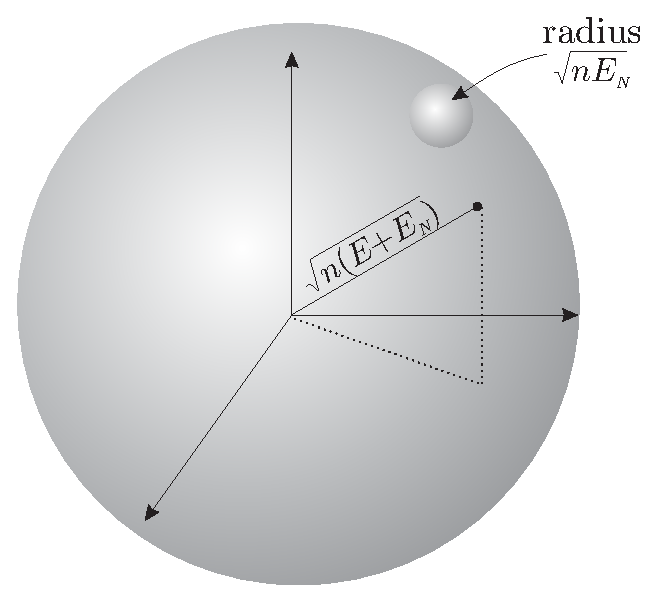
\includegraphics[width=0.5\textwidth]{../images/sphere_in_sphere.eps}}
  \caption{Shannon's capacity formulation simplifies to the geometrical question of: how many hyperspheres of a smaller radius $\sqrt{nE_N}$ fit into a hypersphere of radius $\sqrt{n(E + E_N)}$?}
  \label{F:sphere_in_sphere}
\end{figure}


Keep in mind that the number $M$ is the number of different symbols in the constellation diagram, that is, the number of different messages that could have been sent in $n$ pulses.  

Again, the problem has reduced to: how many hyperspheres of a smaller radius $\sqrt{nE_N}$ fit into a hypersphere of radius $\sqrt{n(E + E_N)}$?  We don't have an exact answer, really -- we just find $M$ by dividing the volume of the large hypersphere by the volume of the smaller hypersphere and saying that $M$ \emph{couldn't} be any bigger than that.   Using that approach,
\begin{equation} \label{E:ShannonsM}
  M \le \left( 1 + \frac{E}{E_N}\right)^{n/2}
\end{equation}

\subsubsection{Returning to Hartley}
Adjusting Hartley's formula, if we could send $M$ messages now in
$n$ pulses (rather than 1 pulse) we would adjust capacity to be:
\[
   R_{max} = \frac{2B}{n}  \log_2 M
\]
Using the $M$ from (\ref{E:ShannonsM}) above,
\begin{equation}
   R_{max} \le \frac{2B}{n} \frac{n}{2} \log_2 \left( 1 + \frac{E}{E_N}\right)
   = B \log_2 \left( 1 + \frac{E}{E_N}\right)
     \nonumber
\end{equation}

\subsubsection{Final Results}

Since energy is power multiplied by time, $E=P T_s = \frac{P}{2B}$ where
$P$ is the maximum signal power and $B$ is the bandwidth, and $E_N =
N_0/2$, we have the Shannon-Hartley Theorem,
\begin{equation} \label{E:ShannonHartley2}
  R_{max} \le B \log_2 \left( 1 + \frac{P}{N_0 B}\right).
\end{equation}

This result says that \textbf{a communication system can operate at
bit rate} $R_{max}$ (in a bandlimited channel with width $B$ given power
limit $E$ and noise value $N_0$), \textbf{with arbitrarily low
probability of error.} 

Note that $R_{max}$ is often called $C$ for ``capacity'', but as we already used $C$ for received power, I'm using $R_{max}$.

Shannon also proved that any system which operates at a bit rate
higher than the capacity, that is, $R_b > R_{max}$, will \emph{certainly} incur a positive bit error rate. Any reliable communication system should thus operate at $R_b < R_{max}$, where $R_b$ is the operating bit rate.

Note that the ratio $\frac{E}{N_0 B}$ is the signal power divided by
the noise power, or signal to noise ratio (SNR).  Thus the capacity
bound is also written $R_{max} \le B \log_2 ( 1 + SNR )$.


\subsection{Efficiency Bound}

Another way to write the maximum signal power $P$ is to multiply it
by the bit period and use it as the maximum energy per bit, \ie,
$\En_b = P T_b$. That is, the energy per bit is the maximum power
multiplied by the bit duration. Thus from (\ref{E:ShannonHartley2}),
\begin{equation}
  R_{max} \le B \log_2 \left( 1 + \frac{\En_b / T_b}{N_0 B}\right) \nonumber
\end{equation}
or since $R_b = 1/T_b$,
\begin{equation}
  R_{max} \le B \log_2 \left( 1 + \frac{R_b}{B} \frac{\En_b}{N_0}\right) \nonumber
\end{equation}
Here, $R_{max}$ is just a capacity limit.  Be know that our bit rate $R_b
\le R_{max}$, so
\begin{equation}
  \frac{R_b}{B} \le \log_2 \left( 1 + \frac{R_b}{B} \frac{\En_b}{N_0}\right) \nonumber
\end{equation}
Defining $\eta=\frac{R_b}{B}$ (the spectral efficiency),
\begin{equation}
  \eta \le \log_2 \left( 1 + \eta \frac{\En_b}{N_0}\right) \nonumber
\end{equation}
This expression can't analytically be solved for $\eta$.  However,
you can look at it as a bound on the bandwidth efficiency as a
function of the $\frac{\En_b}{N_0}$ ratio.  This relationship is
shown in Figure \ref{F:Bound-Bandwidth-Efficiency}.  Figure
\ref{F:Bound-Bandwidth-Efficiency-2} is the plot on a log-y axis
with some of the modulation types discussed this semester.


\begin{figure}[htbp]
  \centerline{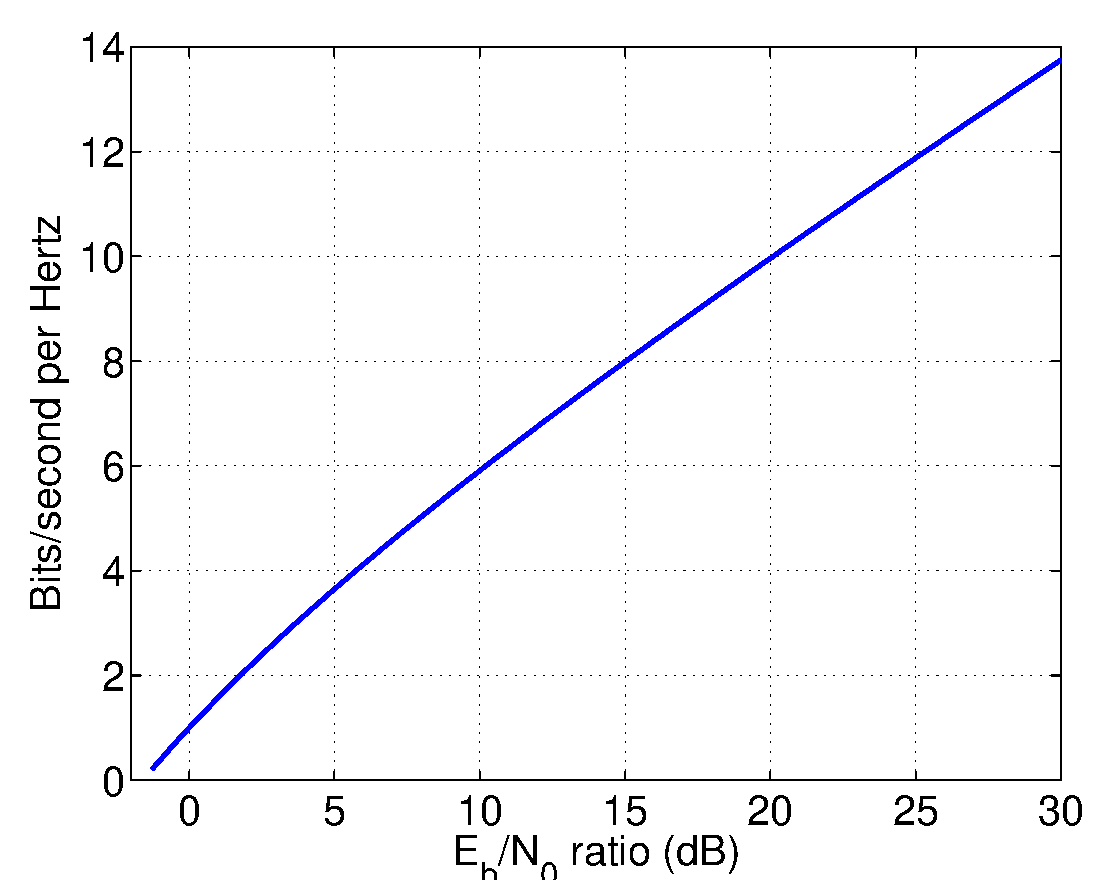
\includegraphics[width=3.5in]{../images/plotShannonEfficiencyBoundLinear.eps}}
  \caption{From the Shannon-Hartley theorem, bound on bandwidth efficiency, $\eta$.}
  \label{F:Bound-Bandwidth-Efficiency}
\end{figure}
\begin{figure}[htbp]
  \centerline{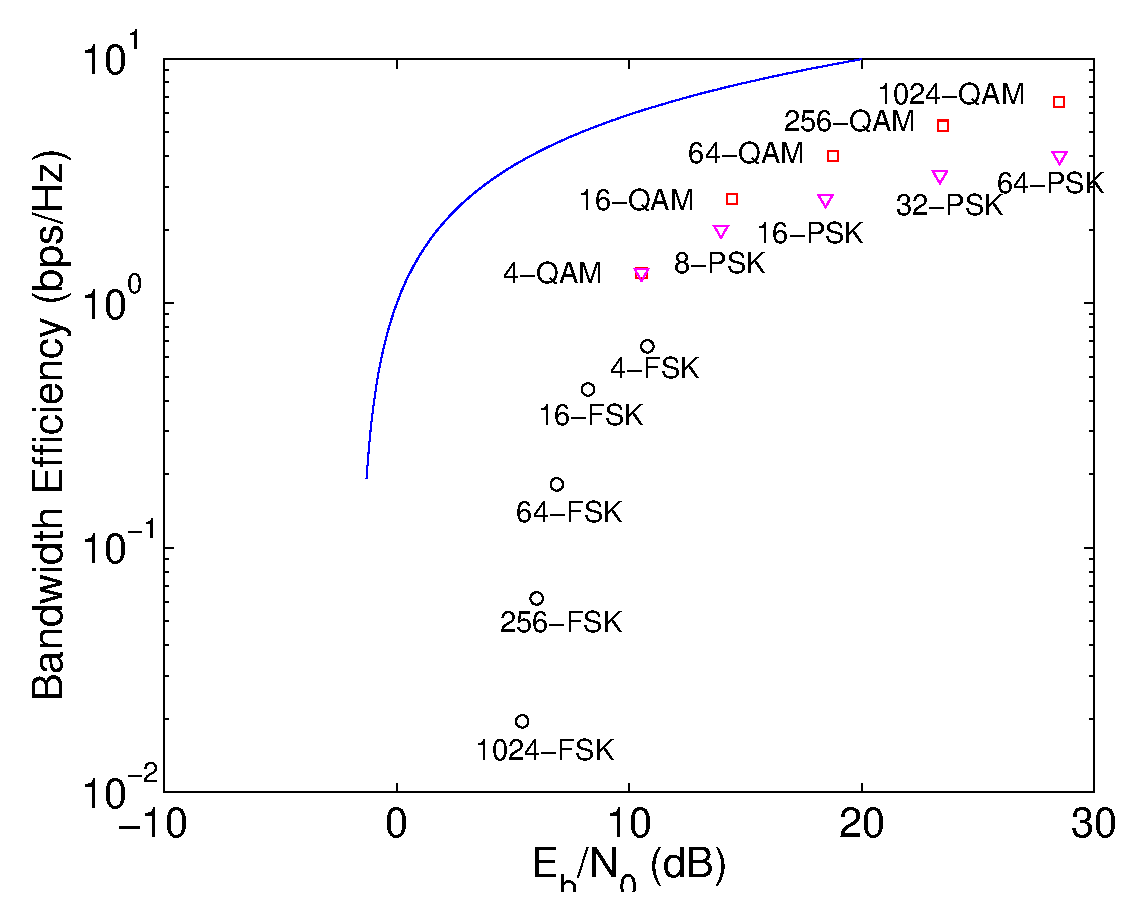
\includegraphics[width=4.0in]{../images/plotShannonWithModTypes.eps}}
  \caption{From the Shannon-Hartley theorem bound with achieved bandwidth efficiencies of M-QAM, M-PSK, and M-FSK.}
  \label{F:Bound-Bandwidth-Efficiency-2}
\end{figure}


\section{Forward Error Correction Coding}

As a result of Shannon's capacity theorem, you can see that the modulations we've covered to this point do not get very close to the bandwidth efficiency limit.  In fact, the  modulations we've covered are within 6-10 dB in $\Ebno$, or a factor of 2-10 in terms of bandwidth efficiency.   Communications engineers, over the past 50 years, have addressed this gap using advances in forward error correction coding (FEC).  Starting from simple coding schemes which improved provided 1-3 dB of gain in the $\Ebno$, the most recent coding methods (LDPC, Turbo codes) can allow one to nearly achieve Shannon's bound.  

{\bf Additional Resource:} You might be interested in Prof.\ Jeff Frolik's MUSE channel coding video, the source of some of these lecture notes.  It is available at:
\begin{itemize}
 \item \url{http://www.uvm.edu/~muse/CTA.html}
\end{itemize}

\Definition{Forward error correction coding or
channel coding}{Adding redundancy to our data at the transmitter with the purpose of detecting and correcting errors at the receiver.}

The transmitter takes in data bits and puts out coded bits.  Our notation is that for each $k$ data bits input to the FEC operator, the FEC operation will produce $n>k$ coded bits out.

You might complain that FEC appears to do the exact opposite of source coding.  While source coding removed redundancy from the source data, FEC adds redundancy.  The key is that FEC adds the redundancy in a structured way that enables it to correct errors at the receiver.

\subsection{Block vs. Convolutional Coding}

\Definition{$(k,n)$ Block Code}{A $(k,n)$ block code inputs $k$-bits which are accumulated (via serial-to-parallel conversion) in a $k$-length vector $\mbd$.  Block encoding  multiplies $\mbd$ by a $k\times n$ generator matrix, $G$, to output a $n$-length bit vector $\mbc$.  Block decoding then multiplies the received vector $\mbr$ by the syndrome matrix $S$ to determine if any errors occurred and determine which (if any) bits were in error out of the $n$ sent.}

The syndrome is just a rearrangement of the transpose of the generator matrix, as shown by example below.

In contrast, a convolutional code is a ``running'' code.  For encoding, bits are input into what is effectively a binary filter, the output bits are dependent on the current and past bits.

Compare the advantages and disadvantages:
\begin{itemize}
 \item Block codes: Advantages: Better for data that is not coming in large streams (bursty data sources, $<$1000 bits), \eg, wireless sensor networks.  Simple linear block codes are not the best in terms of improving efficiency / removing errors.  Low density parity check (LDPC) codes are a type of block code that can be used to nearly achieve the Shannon capacity limit (\emph{capacity approaching}), and used today in DVB and 802.11n (WiFi n), and 5G.
 \item Convolutional codes:  Advantages: Best for very large data streams.  More energy efficient than block codes when you have large streams of data.  Convolutional codes are used in:  deep space communication (Voyager program), satellite and terrestrial digital video broadcasting.  Disadvantages:  Computational complexity increases exponentially in the length of the code.  Andrew Viterbi (founder of Qualcomm) is credited with the optimal decoder, called the Viterbi algorithm.  Turbo codes are a type of convolutional code that can be used to nearly achieve the Shannon capacity limit, and used today in cellular (3G, 4G) protocols and in deep-space communications.
\end{itemize}
% There is another type of code called a Turbo code, which is currently the best available -- it gets us very close the the theoretical limit.  They were developed in 1993.


\subsection{Block Code Implementation}

\begin{figure}[htbp]
\centering{
  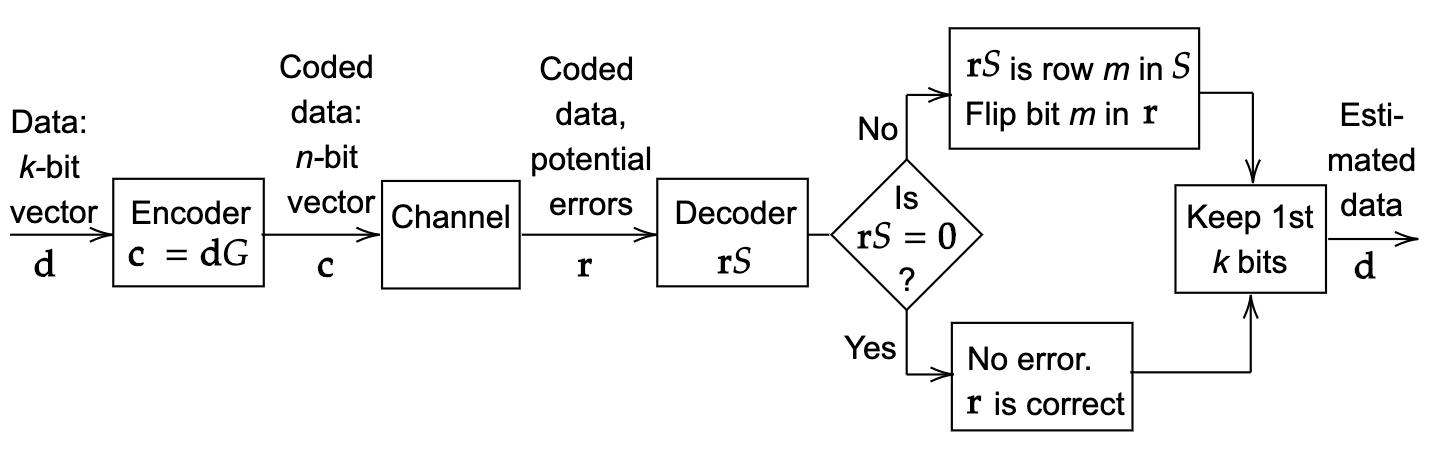
\includegraphics[width=5in]{images/block_coding_decoding_flow_chart_2.png}
}
\caption{The source groups bits into blocks length $k$, and inputs them to the encoding block above.  The channel may introduce error(s). The decoder multiplies each block with a syndrome, and if the result is a vector of all zeros, there is no error.  If not, it looks up the product in the syndrome matrix and finds it in row $m$, and then flips the $m$th bit in $\mbr$.  The final $n-k$ bits are dropped and the remaining $k$ are the received  decoded bits. All products are modulo-2. }
    \label{F:block_coding_flow_chart}
\end{figure}


Let the input be denoted $\mbd$, a $k$-bit vector.
Let the output be $\mbc$, a $n$-bit vector.  Let $G$ be the generator matrix.  Then 
\[
\mbc = \mbd  G
\]
Thus the $G$ matrix has size $k \times n$.  This operation is done modulo-2.  That is, multiply all of the pairs, sum them, and then take the mod 2 of the result.  That is, if the sum of the products is even, the answer is 0, if the sum is odd, the answer is 1.

\Definition{Systematic}{The first $k$ bits of the $n$ bits output, are the same as the $k$ bits in $\mbd$.}

\Example{(6, 3) systematic block code which can correct one bit error} Let $G$ be given by:
\[
G = \left[ \begin{array}{cccccc}
1 & 0 & 0 & 1 & 0 & 1 \\
0 & 1 & 0 & 0 & 1 & 1 \\
0 & 0 & 1 & 1 & 1 & 0 
\end{array} \right]
\]
Encode the data bits $\mbd = [1, 1, 1]$.

Solution: $\mbc  =[ 1, 1, 1, 0, 0, 0]$

\Example{Reception}
You receive $\mbr = [ 1, 1, 1, 0, 0, 1]$, that is, what you received has an error in the last bit compared to $\mbc$ (the coded bits that were sent through the channel).  What was is the block decoder's estimate of the transmitted data?

Solution: At the receiver, multiply by the syndrome 
\[
S = \left[ \begin{array}{ccc}
1 & 0 & 1 \\
0 & 1 & 1 \\
1 & 1 & 0 \\
1 & 0 & 0 \\
0 & 1 & 0 \\
0 & 0 & 1 
\end{array} \right]
\]
Compute: $\mbr S = [ 0, 0, 1]$.

Look at all of the rows of the syndrome.  The row number of the syndrome $S$ that matches the output $\mbr S$, is the same as the number of the bit that was in error.  If $\mbr S$ is all zeros, that indicates that there were no errors.  Since the sixth bit was in error, instead of $[ 1, 1, 1, 0, 0, 1]$, we know the correct coded bits were $[1, 1, 1, 0, 0, 0]$.

Finally, because it is a systematic code, we know the first three bits are the data bits.  The receiver will just drop the last three bits.

\Example{(7, 4) Block Code}
\begin{enumerate}
 \item Encode $\mbd = [0,1,1,0]$ with the $(7,4)$ block code with generator,
\[
G = \left[ \begin{array}{ccccccc}
1 & 0 & 0 & 0 & 1 & 1 & 1 \\
0 & 1 & 0 & 0 & 0 & 1 & 1 \\
0 & 0 & 1 & 0 & 1 & 0 & 1 \\
0 & 0 & 0 & 1 & 1 & 1 & 0 
\end{array} \right]
\]
\item If $\mbr = [0,1,1,0,1,1,1]$ is received, and $S$ is given as below, what would the receiver determine to be the demodulated bits?
\[
S = \left[ \begin{array}{cccc}
1 & 1 & 1 \\
0 & 1 & 1 \\
1 & 0 & 1 \\
1 & 1 & 0 \\
1 & 0 & 0 \\
0 & 1 & 0 \\
0 & 0 & 1 \\
\end{array} \right]
\]
\item If $\mbr = [0, 0, 0, 1, 1, 1, 0]$ is received, what would the receiver determine to be the demodulated bits?

\item If $\mbr = [1, 0, 0, 1, 1, 1, 0]$ is received, what would the receiver determine to be the demodulated bits?

\item If $\mbr = [1, 1, 0, 1, 1, 1, 0]$ is received, what would the receiver determine to be the demodulated bits?
\end{enumerate}

% \mbd = [0 1 1 1].  Then \mbd G = [0 1 1 1 0 0 0].
% \mbd = [0 0 0 1].  Then \mbd G = [0 0 0 1 1 1 0].
% \mbd = [0 0 1 1].  Then \mbd G = [0 0 1 1 0 1 1].

\Solution{ (1) I get $\mbc = [0,1,1,0,1,1,0]$.  (2) Then, multiplying $[0,1,1,0,1,1,1] S$,
I get $[0, 0, 1]$, which is the same as the 7th row, which says that the last row was incorrectly received, and so the 7th bit was incorrect.  Thus the correct four bits sent were $[0, 1, 1, 0]$. (3) I get $\mbr S = [ 0, 0, 0]$ which means no bits were received in error, so the four data bits sent were $[0, 0, 0, 1]$. (4) I get $\mbr S = [ 1, 1, 1]$ which means that the first bit was received in error, so the four data bits sent were $[0, 0, 0, 1]$. (5) I get $\mbr S = [ 1, 0, 0]$ which means that the receiver thinks the fifth bit was received in error, so the receiver would guess the four data bits were $[1, 1, 0, 1]$.}

\subsection{Performance and Costs}

Using a (7,4) block code, we can correct a single error in the seven bits.  But we need to increase the number of bits to send, which then requires more energy.  So when using channel coding, we reduce the transmit power such that the total energy is identical to transmitting the four uncoded bits.  This allows an `equal-energy' comparison of uncoded and coded transmissions.  Still, the probability of bit error goes down for equal $\Ebno (\mbox{dB})$.  Equivalently, we can achieve the same bit error rate at 1 dB lower $\Ebno$.  This value, 1 dB, is the \textit{coding gain}.  In our link budgets, coding goes in the Gains column, added in with the antenna gains.

However, coding requires sending additional bits.  So, in a coded system, there is always a ratio of data bits to coded bits, $r$, called the \textit{code rate}.  In the (7,4) block code it is $r = 4 \mbox{ data bits } / 7 \mbox{ coded bits}$.  For a fixed bandwidth, this reduces the achievable data rate by $r$.  For a fixed data rate, it increases the bandwidth by a factor of $1/r$.

\subsection{For more information}

Looking forward to other material not covered here: A semester-long graduate course in error correction coding would teach you more algorithms to use to code and decode block and convolutional codes.  Such algorithms and coding methods form the basis for the best codes we have today, such as LDPC codes, polar codes, and turbo codes. 